%%%%%%%%%%%%%%%%%%%%%%%%%%%%%%%%%%%%%%%%%
% Dreuw & Deselaer's Poster
% LaTeX Template
% Version 1.0 (11/04/13)
%
% Created by:
% Philippe Dreuw and Thomas Deselaers
% http://www-i6.informatik.rwth-aachen.de/~dreuw/latexbeamerposter.php
%
% This template has been downloaded from:
% http://www.LaTeXTemplates.com
%
% License:
% CC BY-NC-SA 3.0 (http://creativecommons.org/licenses/by-nc-sa/3.0/)
%
%%%%%%%%%%%%%%%%%%%%%%%%%%%%%%%%%%%%%%%%%
% Amended by Evan Russenberger-Rosica 6/14/2019
%

%----------------------------------------------------------------------------------------
%	PACKAGES AND OTHER DOCUMENT CONFIGURATIONS
%----------------------------------------------------------------------------------------

\documentclass[8pt,final,hyperref={pdfpagelabels=false}]{beamer}
\usepackage{multirow}
\usepackage[orientation=landscape,size=a0,scale=1.4]{beamerposter} % Use the beamerposter package for laying out the poster with a portrait orientation and an a0 paper size
\usepackage{xcolor}
\usetheme{I6pd2} % Use the I6pd2 theme suplied with this template
%\usepackage{extsizes}
\usepackage[english]{babel} % English language/hyphenation

\usepackage{amsmath,amsthm,amssymb,latexsym, subfig} % For including math equations, theorems, symbols, etc
\theoremstyle{plain}

%\usepackage{times}\usefonttheme{professionalfonts}  % Uncomment to use Times as the main font
%\usefonttheme[onlymath]{serif} % Uncomment to use a Serif font within math environments

\usepackage{booktabs} % Top and bottom rules for tables

\graphicspath{{figures/}} % Location of the graphics files

\usecaptiontemplate{\small\structure{\insertcaptionname~\insertcaptionnumber: }\insertcaption} % A fix for figure numbering

%----------------------------------------------------------------------------------------
%	TITLE SECTION 
%----------------------------------------------------------------------------------------

\title{\huge Handwritten Digits Recognition using HOG features and SVM} % Poster title

\author{Imaan Saleem bcsf20m523  \texorpdfstring{\\}{} Tuba Mushtaq bcsf20m550} % Author(s)




\institute{Faculty of Computing and Information Technology} % Institution(s)



%----------------------------------------------------------------------------------------
%	FOOTER TEXT
%----------------------------------------------------------------------------------------

\newcommand{\leftfoot}{  } % Left footer text

\newcommand{\rightfoot}{ Handwritten Digits Recognition using HOG features and SVM} % Right footer text

%----------------------------------------------------------------------------------------

\begin{document}

\addtobeamertemplate{block end}{}{\vspace*{2ex}} % White space under blocks

\begin{frame} % The whole poster is enclosed in one beamer frame

\begin{columns}[t] % The whole poster consists of four major columns, each of which can be subdivided further with another \begin{columns} block - the [t] argument aligns each column's content to the top

% --------------------------- BEGIN COLUMN 1 ----------------------------------------------
\begin{column}{.23\textwidth} % The first column. Since there are 4 columns each col width must be less than 1/4 = .25 wide
                
    \begin{block}{Introduction:}
        \begin{itemize}
            \item
            Handwriting recognition is the ability of a computer to receive and
interpret intelligible handwritten input from sources such as paper
documents, photographs, touch-screens, and other devices. There
are many techniques to that have been developed to recognize the
handwriting. One of them is Optical character recognition. 
            
            \item Algorithms:
Machine learning establishes classification methods are K-Nearest Neighbor (KNN), Decision Tree (DT), and Neural Networks (NN). In this experiment, we will discuss the handwritten digits classification using Histogram of Oriented Gradient (HOG) features and a Support Vector Machine (SVM) analyzed on MNIST dataset.
        \end{itemize}
    \end{block}
    
    \begin{block}{HOG and SVM}
        \begin{itemize}
            \item Histogram of Oriented Gradients (HOG):The histogram of oriented gradients (HOG) is a feature descriptor used in computer vision and image processing for the purpose of object detection.
            
            \item Support vector machines (SVM):Support vector machines (SVMs) are a set of supervised learning methods used for classification, regression and outliers detection.

        \end{itemize}
    \end{block}
    
    \begin{block}{MINIST dataset:}
        \begin{itemize}
            \item MNIST is a widely used dataset for the hand-written digit classification task. It consists of 70,000 labeled 28x28 pixel grayscale images of hand-written digits. MNIST is one of the most famous and popular used database for handwritten digits recognition which contains 70,000 samples included two parts of 60,000 and 10,000 samples corresponding to training and test data.From the total numbers of instances, Some of the samples are shown in figure 1
            \vspace{\baselineskip} 
             
           \begin{figure}
                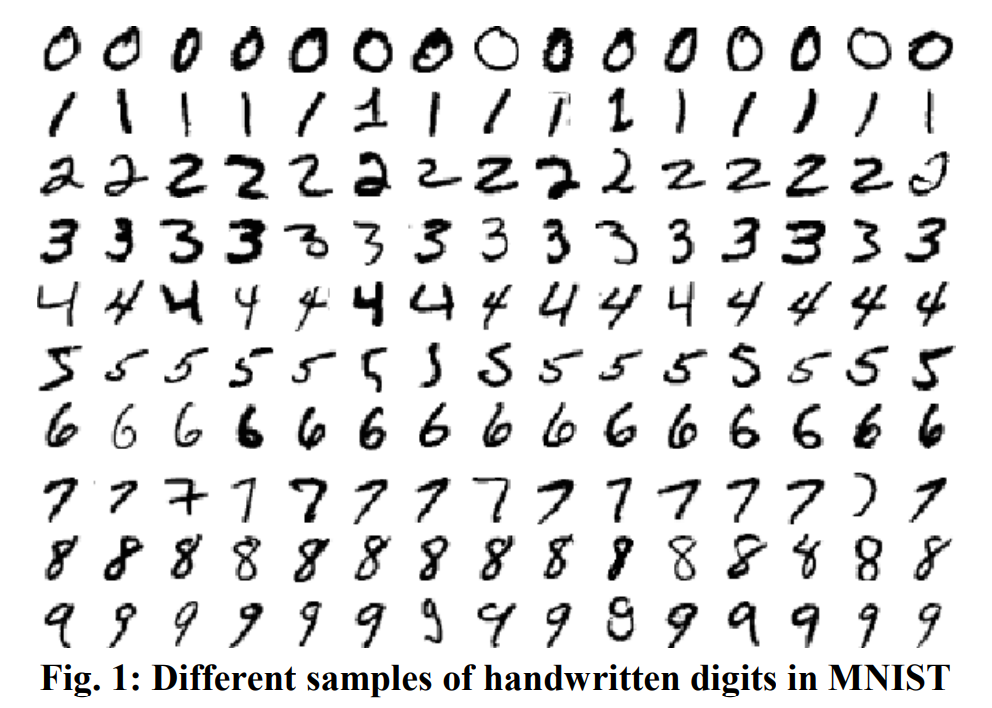
\includegraphics[width=.8\linewidth]{figures/samples of handwritten digits.png}
            \end{figure}
        \end{itemize}
    \end{block}

\end{column} % End of the first column
 
% --------------------------- BEGIN COLUMN 2 ----------------------------------------------
\begin{column}{.23\textwidth} % The second column
    
    \begin{block}{Procedure}
        \begin{itemize}
        \item There are 10 classes corresponding to the handwritten digits from ‘0’ to ‘9’ which are very depend on the handwritten. The main difficulty in the handwritten digit’s recognition is different handwritten style which is a very personal behaviour where there are a lot of models for numbers based on the angles, length of the segments, stress on some parts of numbers. Figure 1 shows 15 different handwritten digits related to these issues. However, recognizing numbers is clear for human but it is not very easy for machines especially when there are some ambiguities on different classes (e.g., ‘1’ and ‘7’).
        
         \item When collecting a data set we will split it into two parts: one for training and the other for testing.
        
        \end{itemize}
    \end{block}
    
    \begin{block}{Training and Testing}
        \begin{itemize}
        
            \item There are different methods for splitting the dataset, the most common following the Pareto ratio of 80:20 or 70:30. 
        
            \item Training data is a set of samples (such as a collection of photos or a set of texts) with assigned relevant and comprehensive labels (classes or tags) used to fit the parameters (weights) of a machine learning model with the goal of training it.We will use 80\% of data for training.
            
            \item After we have trained the machine learning model, we will use the 20\% of saved from the training data set to test it.
            
        \end{itemize}
    \end{block}
    
    \begin{block}{Description on whole model:}
        \begin{itemize}
        
            \item Our model works in three steps: \\ 1) Preprocessing, \\ 2) HOG features extraction and \\ 3) Support vector machines classification. \\ 
            \item In the preprocessing, we have some basic image processing to separate numbers from real samples or preparing data from dataset (which is reshaped from images to the vectors)
            
            \item In the second part, we extract HOG features which is very distinguishable descriptor for digits recognition where we divide an input image into 9×9 cells and compute then the histogram of gradient orientations thereby we represent each digit with a vector of 81 features. 
            
            \item In the third stage, a linear multiclass support vector machine has been employed to classify digits. 
             \item In general, the main contribution of our model is employing HOG features with SVM. HOG can perform distinguishable features. And SVM can be useful to classify HOG features.
        
        \end{itemize}
    \end{block}
    
\end{column} % End of the second column

% --------------------------- BEGIN COLUMN 3 ----------------------------------------------
\begin{column}{.23\textwidth} % The Third column
    
        \begin{block}{Overall Structure}
        \begin{itemize}
        
            \item The overall view of proposed approach has been illustrated in Figure 2.
            %\vspace{\baselineskip} 
            \begin{figure}
                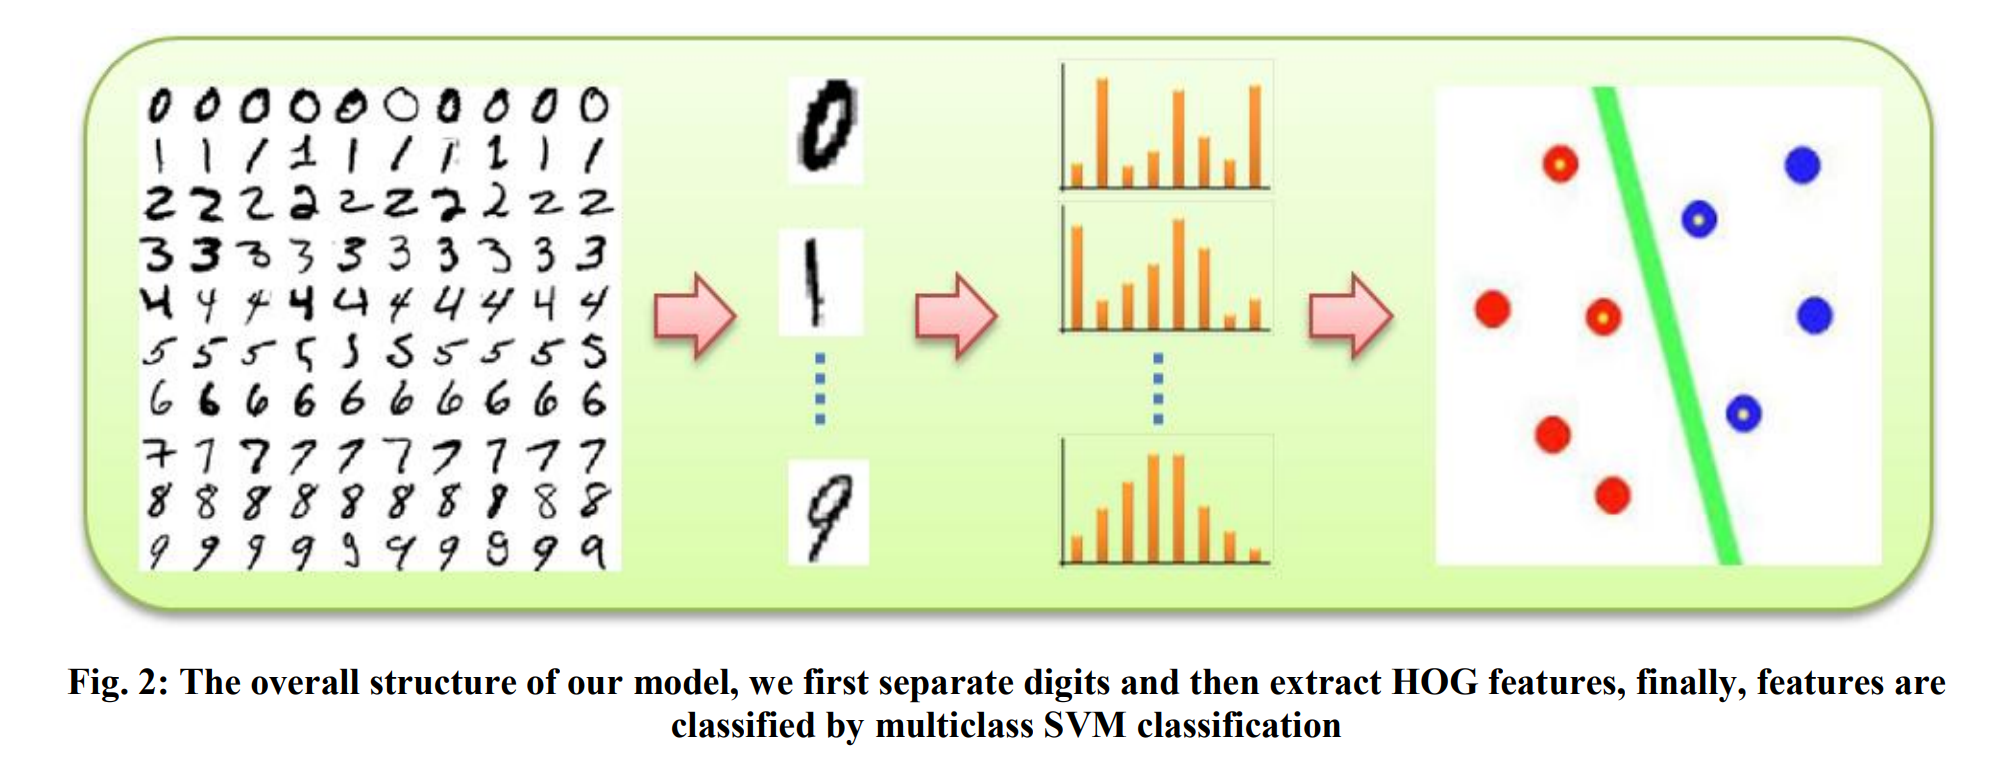
\includegraphics[width=.8\linewidth]{figures/HOG and SVM.png}
            \end{figure}
            
            \item The total numbers of instances are shown in Table 1 ordered by classes.
            %\vspace{\baselineskip}
            
            \begin{figure}
                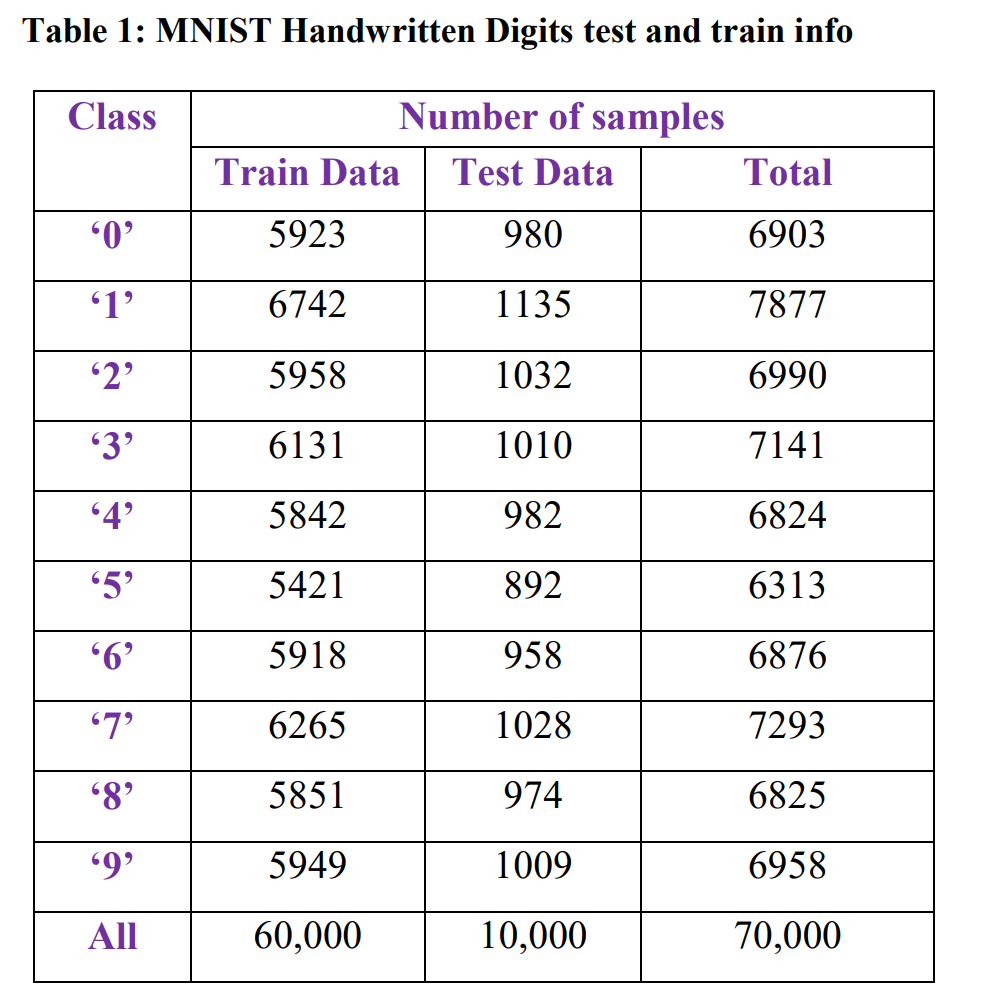
\includegraphics[width=.8\linewidth]{figures/test train info.png}
            \end{figure}
            
            \item Applying testing digit to the trained model  
            \vspace{\baselineskip}
            
            \begin{figure}
                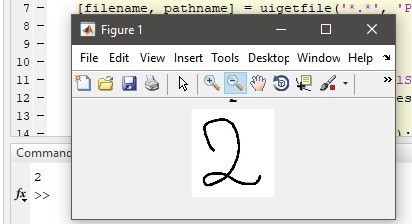
\includegraphics[width=.8\linewidth]{figures/resultfinal.jpeg}
            \end{figure}
        
        \end{itemize}
    \end{block}
    
    \begin{block}{Conclusion}
        
        \begin{itemize}
            \item In general, proposed approach used HOG which is a very efficient appearance-based descriptor with linear multiclass SVM classification for handwritten digits recognition. We have successfully done digit recognition using this method. The most important benefit of above structure is that our model is fast and useful for real-time applications.
            
        \end{itemize}
    \end{block}
\end{column} % End of the Third column

% --------------------------- BEGIN COLUMN 4 ----------------------------------------------
\begin{column}{.23\textwidth} % The Fourth column
    \begin{block}{Matlab Code}
    
     \begin{itemize}
            \item Training Code\\
            \vspace{\baselineskip}
            clc;\\
    clear all;\\
    close all;\\
    warning off;\\
    imds=imageDatastore('database','IncludeSubFolders',true,\\'LabelSource','foldernames');\\
    trainingFeatures=[];\\
    trainingLabels=imds.Labels;  \\     
    for i = 1:numel(imds.Files)\\         % Read images using a for loop
        img = readimage(imds,i);\\
        trainingFeatures(i,:) = extractHOGFeatures(img,'CellSize'\\,[8 8]);\\
    end\\
    Classifier =fitcecoc(trainingFeatures,trainingLabels);\\
    save Classifier Classifier\\
    \vspace{\baselineskip}

            
        \end{itemize}
       
       \begin{itemize}
            \item Test Code\\
            \vspace{\baselineskip}
            clc;\\
    clear all;\\
    close all;\\
    warning off;\\
    load Classifier;\\
   {[filename, pathname]} = uigetfile('*.*', 'Pick an Image');\\
    filename=strcat(pathname,filename);\\
    imga=imread(filename);\\
    img=imresize(imga,[45 24]);\\
    {[Features]} = extractHOGFeatures(img,'CellSize',[8 8]);\\
    PredictedClass=predict(Classifier,Features);\\
    PredictedClass=char(PredictedClass);\\
    figure,\\imshow(imga),title(PredictedClass);\\
    disp(PredictedClass);\\

            
        \end{itemize}

       
    \end{block}
    \begin{block}{References}
        
        \begin{itemize}
            \item International Journal of Computer Applications (0975 – 8887) Volume 104 – No.9, October 2014 
            
            \item 	https://medium.com/@basu369victor/handwritten-digits-recognition-d3d383431845
            
            \item 	https://labelyourdata.com/articles/machine-learning-and-training-data
            
             \item https://www.analyticsvidhya.com/blog/2019/09/feature-engineering-images-introduction-hog-feature-descriptor/
        \end{itemize}
    \end{block}

\end{column} % End of the Fourth column
\end{columns} % End of all the columns in the poster
\end{frame} % End of the enclosing frame

\end{document}